\section{Instance Pointcuts for Program Comprehension} 
\label{sec:ipc:cocos}
Complex software systems are difficult to understand because they consist of many elements with complicated dependencies.
A factor further complicating the comprehensibility is the dynamicity of execution semantics:
In object-oriented programming languages, the dynamic type of the receiver object determines which implementation of the called method will be executed.
It is generally not possible to determine the dynamic type of an expression just by looking at the source code.
For this reason, often dynamic tools are used to observe the program execution for comprehending a program.
As such tools are mainly used during debugging, they are often called \emph{debuggers};
we will also use this term throughout this paper to refer to tools which in general allow observing and possibly interacting with program executions at runtime.

In object-oriented programming, on the source code level the main abstractions are classes (object-oriented languages which are not class-based provide an equivalent like prototypes in delegation-based languages).
At runtime, however, the main building blocks are \emph{objects} which are instances of classes.
Comprehending the behavior of a program means to comprehend the interplay of objects.
In general, there can be arbitrarily many instances of each class, which makes the comprehension difficult as their connections and dependencies can be manifold.

A natural technique to increase comprehensibility is introducing a limited number of categories, grouping all objects into categories and considering only the categories during the comprehension task.
This is even well supported by object-oriented languages, since classes already form such categories and there is an easily observable relation between an object and its class, and vice versa.
However, the categorization offered by the class structure of the program is not always the best fit for the comprehension task at hand.
On one hand, instances of the same class may be used in different ways throughout the program execution; on the other hand, instances of different classes may be used in the same or a similar way.

For these reasons, we claim that another, more powerful and flexible way for dynamically categorizing objects is needed to guide the task of program comprehension.
In our ongoing research, we are developing the language concept of \emph{instance pointcuts}, originally to facilitate flexibly extending program behavior and composing independently developed architectural components.
Recently, we have found the abstraction provided by instance pointcuts also to be useful to support comprehension of highly dynamic object-oriented programs.


Using pointcut-based techniques for specifying breakpoints in a debugger has been proposed before.
For example, Chern and De Volder \cite{Chern2007} have proposed to define breakpoints based on the current control flow, similar to AspectJ's \lstinline!cflow! pointcut designator.
Bodden has proposed stateful breakpoint \cite{Bodden2011}, which allows programmers to specify the order in which different events must occur to lead to suspension of the program execution.
Yin et al.\ have presented a language for specifying breakpoints \cite{Yin2013} which is also based on a pointcut language and already allows specifying breakpoints based on object relations.
Nevertheless, the approach presented in our paper is the first to actually maintain a set of objects, which relate by how they have been used in the past, and to expose these sets to different debugging facilities.


In the following section, we will walk the reader through a few particular comprehension tasks in section \ref{sec:walkthrough}, we will illustrate the applicability of instance pointcuts;
throughout this section we will sketch a user interface that visualizes instance pointcuts.
In section \ref{sec:challenges} we will discuss challenges in realizing the outlined concepts.
We present related work in section \ref{sec:related-work} before we conclude our position in section \ref{sec:conclusion}.

\subsection{Example Walkthrough}
\label{sec:walkthrough}

\begin{figure*}[t!]
\begin{minipage}[t]{0.3333\textwidth}
\centering
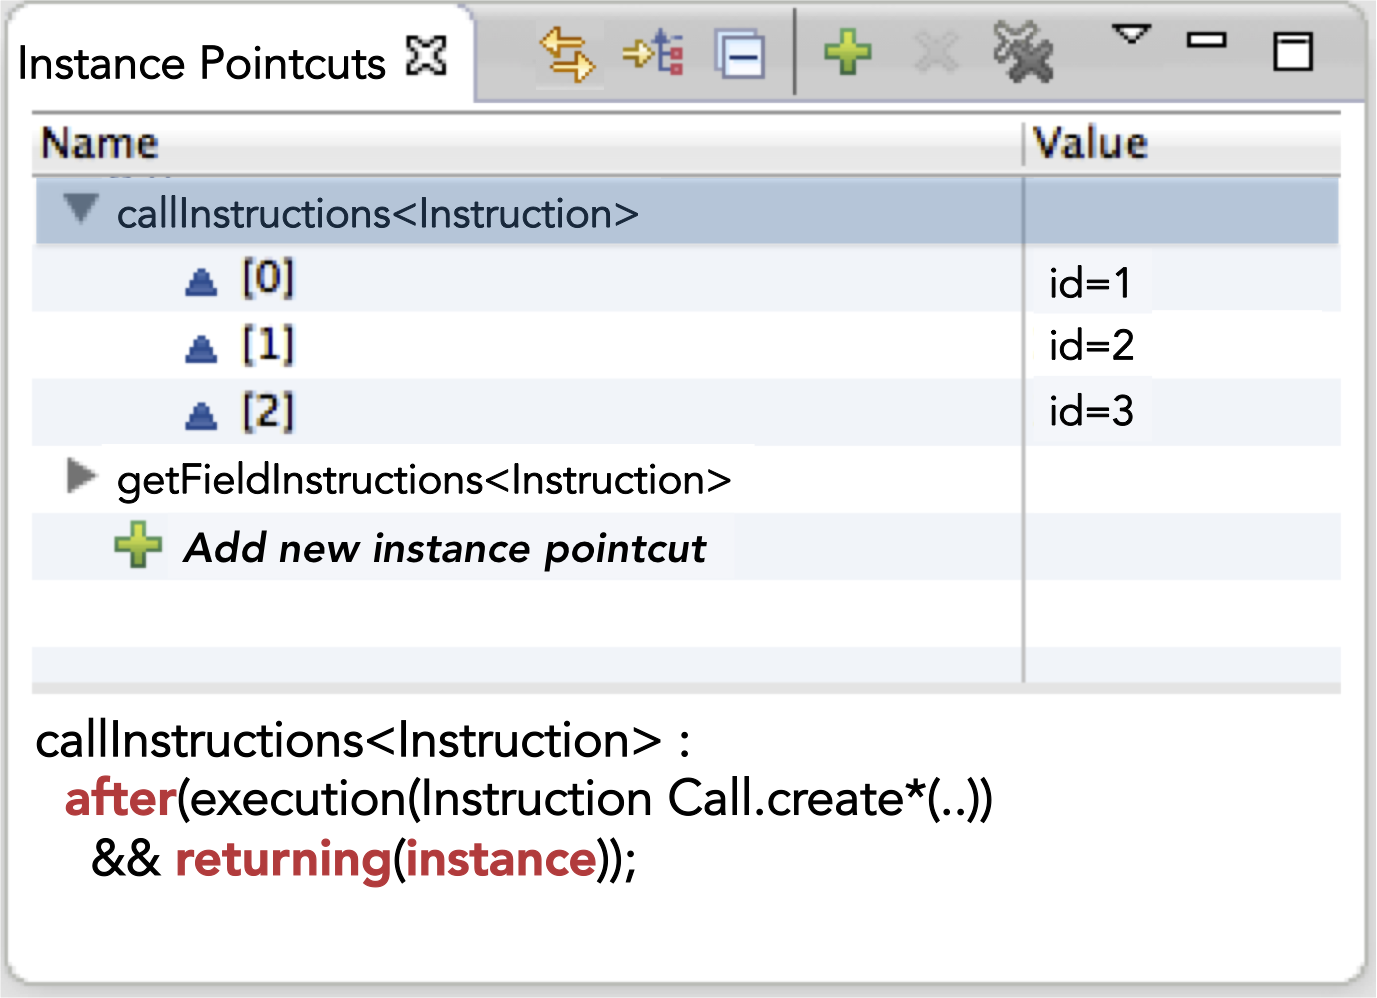
\includegraphics[scale=0.24]{images/callInstructions.png}
\caption{The Instance Pointcuts View}
\label{fig:ip-view}
\end{minipage}
\begin{minipage}[t]{0.3333\textwidth}
\centering
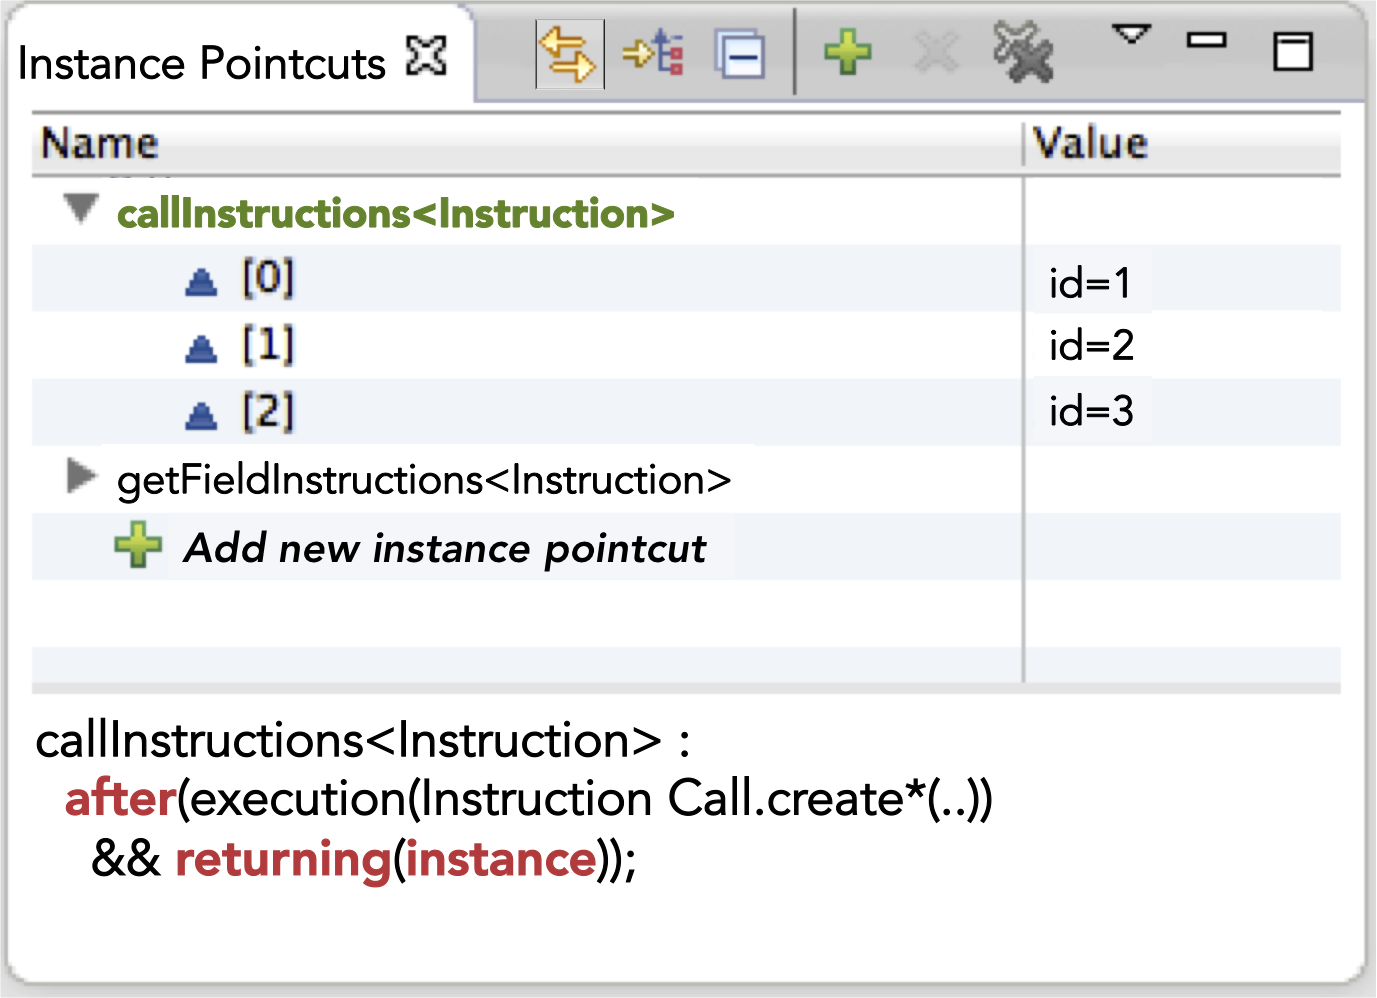
\includegraphics[scale=0.24]{images/callInstructionsHighlighted.png}
\caption{A highlighted instance pointcut.}
\label{fig:ip-view-highlight}
\end{minipage}
\begin{minipage}[t]{0.3333\textwidth}
\centering
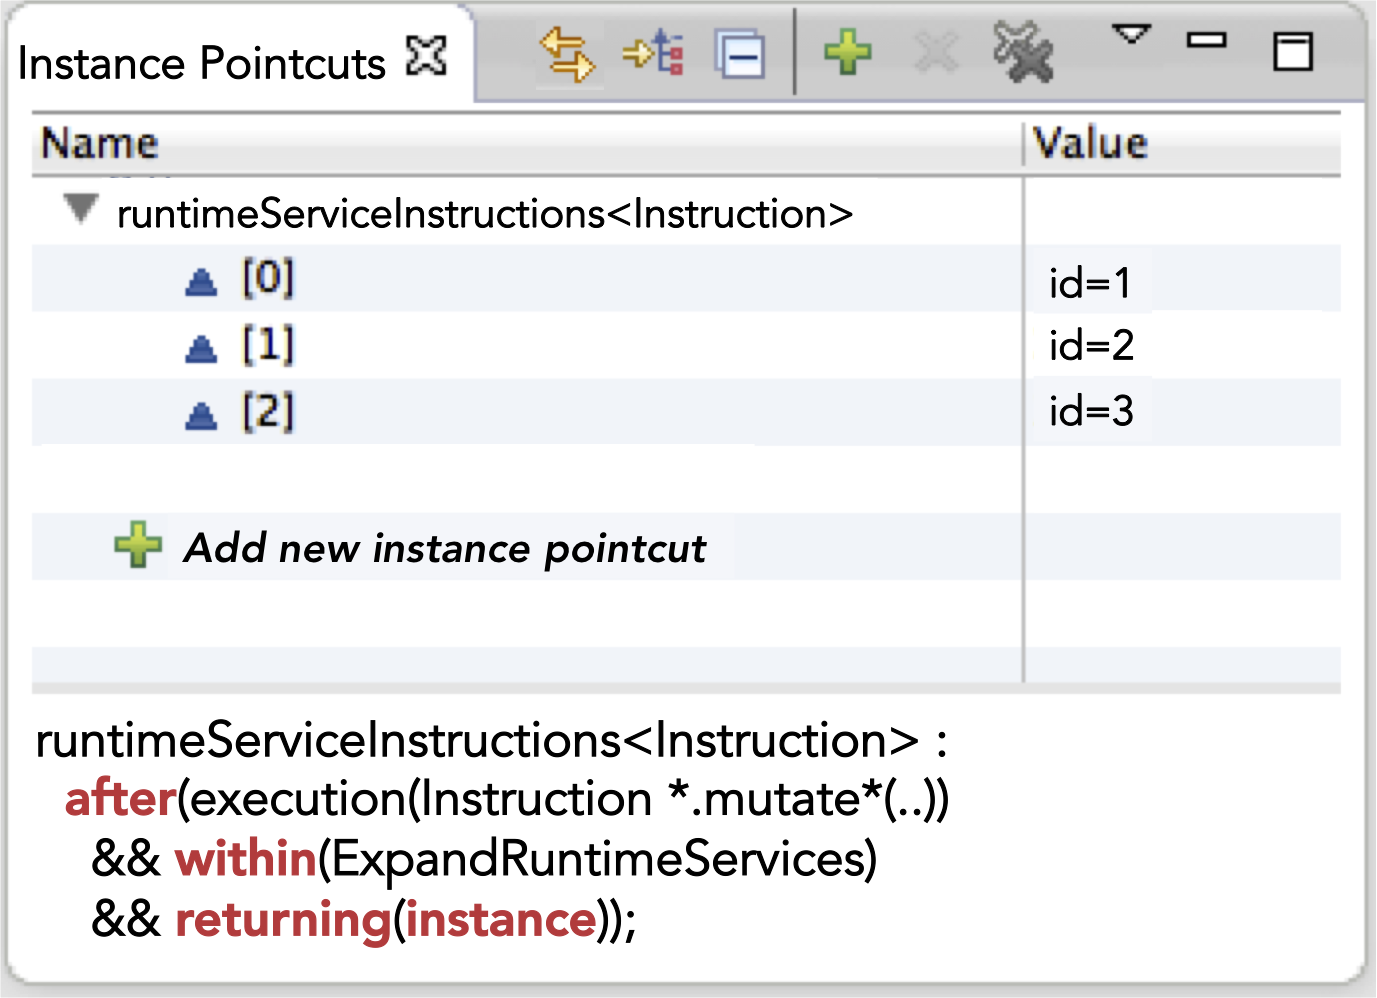
\includegraphics[scale=0.24]{images/runtimeServices.png}
\caption{Another example of an instance pointcut definition.}
\label{fig:ip-view-runtimeServices}
\end{minipage}
\end{figure*}

In this section, we will describe an existing system and several comprehension scenarios where instance pointcuts can be useful.
Intertwined with these scenarios, we will discuss a hypothetical extension to the Eclipse debugger for using instance pointcuts.

We made the observation that instance pointcuts can support program comprehension while working on an extension to the Jikes Research Virtual Machine~\cite{Alpern2005}.
In particular, we were extending the optimizing just-in-time (JIT) compiler of this virtual machine.
The optimizing compiler works in multiple phases, whereby the first one creates an object-based intermediate representation (IR) from the Java bytecode of the method which is currently compiled.
This IR, basically a linked list of \lstinline!Instruction! objects, is iteratively analyzed and rewritten until eventually machine code is emitted.
In our extension we manipulated this IR by inserting instructions and adding rewrites.
When we made a mistake runtime failures occurred and we had to understand the impact of our extension on the further processing of the JIT compiler, i.e. to identify our fault we had to comprehend a very complex system.

All elements in the IR are instances of the same class (\lstinline!Instruction!) which are configured with an \lstinline!Operator! object determining the behavior of the instruction.
Thus, at first sight it is not clear which instruction is represented by an \lstinline!Instruction! object.
Besides the referenced \lstinline!Operator! object, also the creation site of the \lstinline!Instruction! object allows to draw conclusions about the purpose of an \lstinline!Instruction!: There is a factory class for each kind of instruction.
For instance, if we are only interested in instructions representing a function invocation, we can focus our comprehension task on those \lstinline!Instruction! objects that are returned by a \lstinline!create! method in the class \lstinline!Call!.

\subsubsection{Scenario 1}
\label{sec:scenario-1}

\paragraph{A View for Instance Pointcuts}

An instance pointcut, let's call it \lstinline!callInstructions!, selecting the objects described above can be defined as seen in figure~\ref{fig:ip-view}\footnote{For brevity we only show simple class names.}.
The figure depicts a view for defining instance pointcuts.
The new view allows to add instance pointcuts which are maintained during the execution of the program, and to inspect the content of the defined instance pointcuts while the program execution is suspended at a breakpoint.
The left column shows the names of the defined instance pointcuts.
A row with an instance pointcut can be expanded, for example in the figure the instance pointcut \lstinline!callInstructions! is expanded and its elements are listed.
When a row containing the name of an instance pointcut is selected, the detail pane (at the bottom) shows its definition.
When a row is selected which represents an element of an instance pointcut, the \lstinline!toString()! of the value is shown.

\paragraph{Linking the Instance Pointcut View}

The left-most icon of the toolbar in figure \ref{fig:ip-view-highlight} allows linking the Instance Pointcut View with other debugging-related views.
When linking is turned on and an object is selected on another view, e.g. in the Variables view, all instance pointcuts are highlighted which contain the selected object.
Figure \ref{fig:ip-view-highlight} shows the instance pointcut \lstinline!callInstructions! in green, which means that the user has currently selected an object contained in \lstinline!callInstructions!.
In the outlined comprehension task, this feature makes it simple to identify for each \lstinline!Instruction! object, if it represents an instruction relevant for the task, i.e., for which an instance pointcut was defined.


\subsubsection{Scenario 2}

Besides representing different (virtual) machine instructions, \lstinline!Instruction!s also need to be distinguished by the purpose for which they have been created.
The majority of the instructions are directly compiled from the Java bytecode instructions.
But some instructions have to be inserted into the generated machine code to inject the runtime services offered by the virtual machine, e.g., thread switching, memory management, and profiling for facilitating optimizations.
In our concrete case, some instructions are also generated by our own extension to the virtual machine.

A simple example is insertion of the runtime service for managed memory allocation.
This is done in a compiler phase after the initial creation of the \lstinline!Instruction!-based intermediate representation.
When an instruction representing the allocation of an object is encountered in this phase, the \lstinline!Instruction! is \emph{mutated} by turning it into a Call instruction invoking the virtual machine's function realizing this service.
Figure~\ref{fig:ip-view-runtimeServices} shows the instance pointcut selecting all \lstinline!Instruction!s that inject a runtime service.


\paragraph{Using Instance Pointcuts in Conditions and Expressions}

Besides using instance pointcuts during inspection when the execution is suspended at a breakpoint, defined instance pointcuts can also be used for defining conditional breakpoints.
As an example consider the task of comprehending a late compiler phase.
At this time, many \lstinline!Instruction!s have been mutated for optimization purposes or for injecting runtime services.
But many \lstinline!Instruction!s still simply reflect the functionality directly specified by the Java bytecode instructions.
Assume we want to comprehend the impact of injected runtime services on the liveness analysis, a phase necessary for generating meta-data needed by the garbage collector.
Figure~\ref{fig:breakpoint-properties} shows a screenshot of the breakpoint properties dialog where the condition refers to the instance pointcut defined in figure~\ref{fig:ip-view-runtimeServices}.
The execution is only suspended at this breakpoint when the local variable \lstinline!inst! is selected by the instance pointcut describing the \lstinline!Instruction!s that realize runtime services.
In the same way, watch expressions entered in Eclipse's Expression View can refer to instance pointcuts, simply treating them as \lstinline!java.util.Set!s.

\begin{figure*}
\centering
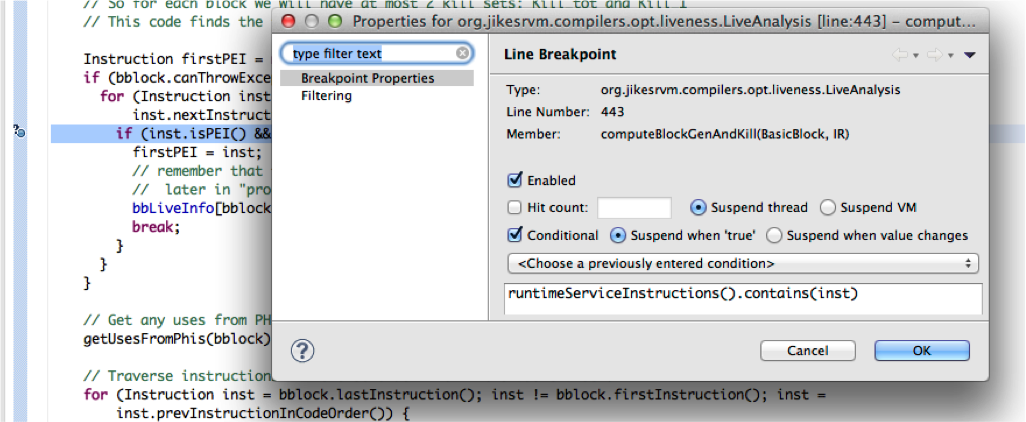
\includegraphics[scale=0.7]{images/breakpointProperties.png}
\caption{Breakpoint properties using an instance pointcut.}
\label{fig:breakpoint-properties}
\end{figure*}

\subsubsection{Scenario 3}

\paragraph{Instance Pointcut Watchpoints}

To demonstrate the \emph{remove expression} feature of instance pointcuts, consider the two scenarios above.
Since mutation changes the operation represented by an \lstinline!Instruction! object, mutated \lstinline!Instruction!s must be removed from the instance pointcut representing a specific operation as mentioned in the first scenario.
Figure~\ref{fig:ip-watchpoints} shows the extended instance pointcut definition.

Furthermore, the language concept of instance pointcuts allows to advise the joint points when a new instance is added to an instance pointcut and when an instance is removed, respectively.
Instance pointcuts internally maintain multisets; we specify that only the initial addition and the final removal of an object are join points, i.e. when the cardinality of an object in the multiset changes from 0 to 1 and from 1 to 0, respectively.
These join points can also be used to define watchpoints.
The two right-most columns in figure~\ref{fig:ip-watchpoints} represent this feature.
In the example, the watchpoint for adding an object to the instance pointcut \lstinline!callInstructions! is enabled; the breakpoint for removing an object is disabled.

\begin{figure}
\centering
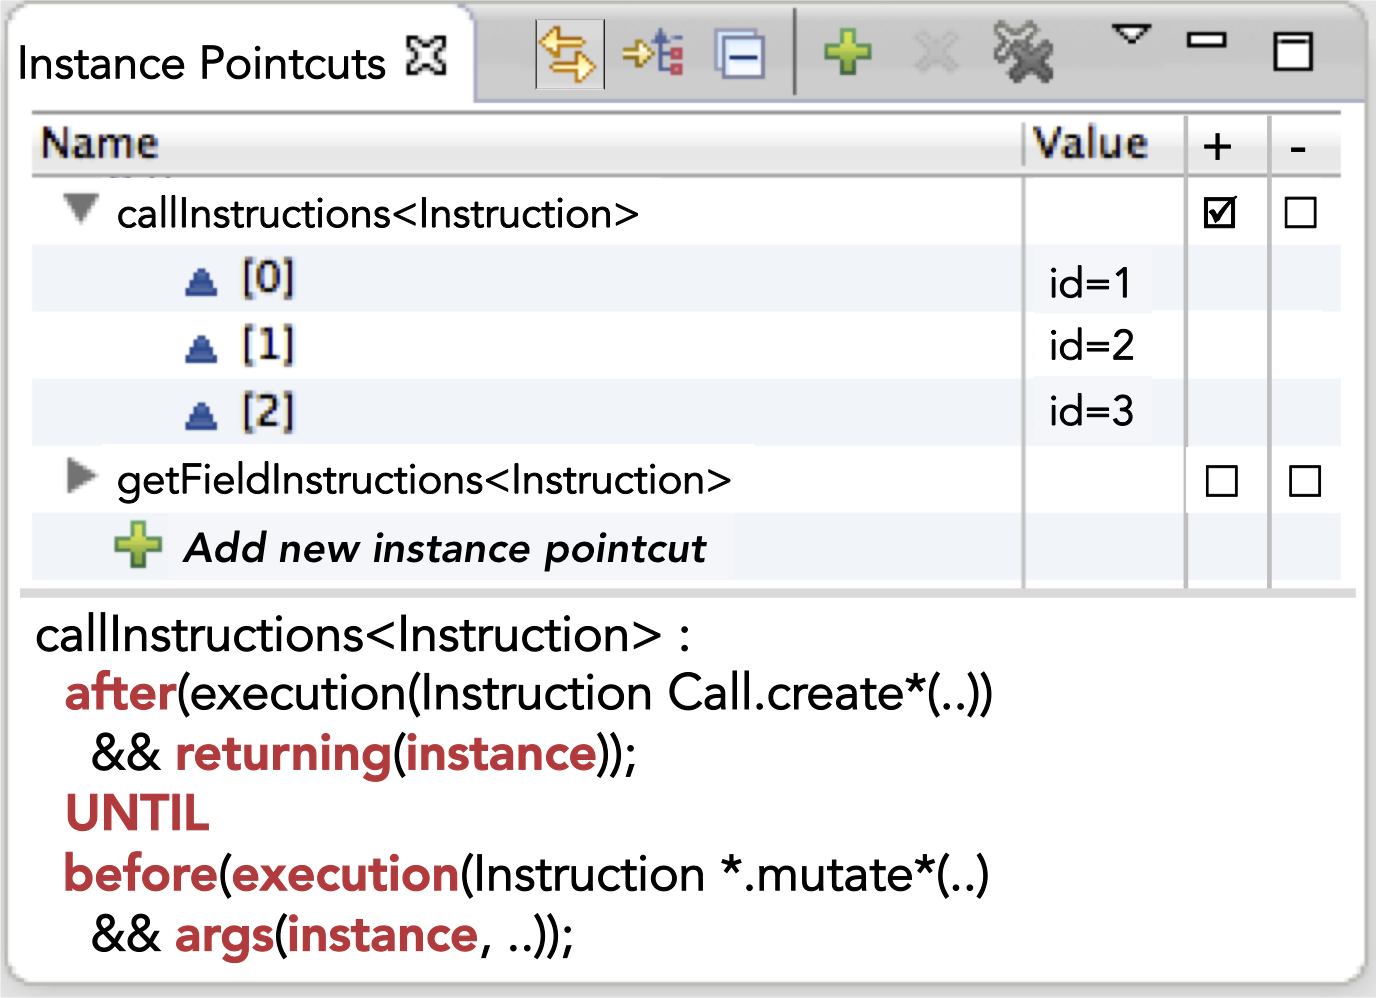
\includegraphics[scale=0.24]{images/callInstructionsUntil.png}
\caption{Setting watchpoints for instance breakpoint changes.}
\label{fig:ip-watchpoints}
\end{figure}

\subsection{Challenges}
\label{sec:challenges}

Obviously, the expressiveness of the pointcut language determines how precisely sets of objects can be selected.
Since in our prototype we use the AspectJ pointcut language underlyingly, we are limited to selecting the supported events and specifying supported restrictions.
In the example of the optimizing compiler of the Jikes virtual machine, this can be a significant limitation:
long switch statements identify different ways of processing instructions and it is often relevant in the context of which \emph{case} an object was used.
However, since AspectJ pointcuts cannot refer to switch cases, they cannot be used in the add or remove expressions of instance pointcuts.

%In the discussion of scenario one (cf.~\ref{sec:scenario-1}) it is apparent that often many similar instance pointcuts have to be defined for a comprehension task, e.g., one instance pointcut per relevant kind of instruction.
%It would be more convenient to define just one instance pointcut and specify the variability, in the example this is the declaring type of the \lstinline!create! method.

We are used to adding breakpoints or watch expressions dynamically, during the runtime of the debugged program.
With instance pointcut, this is not possible or at least risky.
As is always the case with dynamic deployment of aspects, it may be that some relevant join points have already passed at the time of deployment.
Thus, it may be that objects, which should have been selected by an instance pointcut, are not selected; or not all of the recursive additions have been tracked and an object is removed from the multiset too early.
For these reasons, we do not suggest to support dynamic addition of instance pointcuts, even though this may require to restart the program during one comprehension task, if new relevant categorizations for objects are discovered during runtime.




